% Build from doc/: latexmk -pdf -outdir=build/apresentacao apresentacao.tex
\documentclass[aspectratio=169,11pt]{beamer}
\usepackage[T1]{fontenc}
\usepackage[utf8]{inputenc}
\usepackage[brazilian]{babel}
\usepackage{lmodern}
\usepackage{booktabs}
\usepackage{graphicx}
\usepackage{amsmath}
\usepackage{tabularx}

\definecolor{ink}{HTML}{153444}
\definecolor{accent}{HTML}{007F79}
\definecolor{muted}{HTML}{536571}
\setbeamercolor{normal text}{fg=ink,bg=white}
\setbeamercolor{structure}{fg=accent}
\setbeamercolor{frametitle}{fg=ink}
\setbeamercolor{alerted text}{fg=accent}
\setbeamercolor{footline}{fg=muted}
\setbeamerfont{frametitle}{size=\Large,series=\bfseries}
\setbeamerfont{title}{size=\LARGE,series=\bfseries}
\setbeamertemplate{navigation symbols}{}
\setbeamertemplate{itemize items}[circle]
\setbeamersize{text margin left=9mm,text margin right=9mm}
\setbeamertemplate{footline}{%
  \hspace{9mm}\scriptsize Kleber Daniel Mattos Viana
  \hfill Defesa de TCC | UNIFESO | 2026
  \hfill\insertframenumber/\inserttotalframenumber\hspace{9mm}\vspace{3mm}}
\setbeamertemplate{frametitle}{%
  \vspace{4mm}\insertframetitle\par\vspace{2mm}}
\setlength{\tabcolsep}{8pt}
\newcommand{\source}[1]{\par\vspace{2mm}{\tiny\color{muted}#1\par}}
\newcommand{\takeaway}[1]{\par\vspace{3mm}{\color{accent}\bfseries #1\par}}
\newcommand{\evidence}{evidence/v9/figures/}
\hypersetup{
  pdftitle={Defesa de TCC: Detecção de Anomalias e Análise Probabilística},
  pdfauthor={Kleber Daniel Mattos Viana},
  pdfsubject={Defesa de TCC em Ciência da Computação, UNIFESO, 2026}}

\begin{document}

\begin{frame}[plain]
  
\includegraphics[width=2.5cm]{imagens/UNIFESO.png}
  \hfill {\small Defesa de Trabalho de Conclusão de Curso}
  \vspace{5mm}

  {\usebeamerfont{title}Detecção de Anomalias e Análise Probabilística
  em Manobras de Energização de Linhas de Transmissão Utilizando
  Aprendizagem de Máquina\par}
  \vspace{5mm}
  {\large Kleber Daniel Mattos Viana\par}
  \vspace{3mm}
  {\small Bacharelado em Ciência da Computação\par
  Orientadora: Andressa Alves Machado Ruback\par
  Coorientador: Bráulio Chuco Paucar\par}
  \vfill
  {\small Teresópolis, 2026}
\end{frame}

\begin{frame}{Problema de pesquisa}
  \begin{itemize}\setlength{\itemsep}{4mm}
    \item A energização pode produzir sobretensões transitórias.
    \item O ATP gera arquivos extensos; a inspeção manual dificulta
      a organização e a rastreabilidade dos extremos.
    \item Um máximo discrepante pode exigir investigação, mas sua
      raridade não explica sua causa.
  \end{itemize}
  \takeaway{Como selecionar observações discrepantes de forma
    automatizada, reprodutível e rastreável?}
  \source{Fonte: monografia, Introdução. Fundamentação: Dommel (1969);
    Chandola, Banerjee e Kumar (2009).}
\end{frame}

\begin{frame}{Objetivo e escopo}
  \begingroup\large
  Desenvolver uma rotina computacional para extrair, organizar
  e analisar máximos de tensão produzidos pelo ATP.\par
  \endgroup
  \vspace{4mm}
  \begin{itemize}\setlength{\itemsep}{3mm}
    \item Validar os dados e a conversão para por unidade (P.U.).
    \item Descrever distribuições e estimar excedências com incerteza.
    \item Comparar agrupamentos e critérios de candidatos a anomalias.
    \item Preservar o vínculo com a simulação de origem.
  \end{itemize}
  \takeaway{A entrega acadêmica apoia a investigação técnica.}
  \source{Fora do escopo: classificação causal definitiva, exclusão
    automática dos candidatos e recomendação do nível de isolamento.}
\end{frame}

\begin{frame}{Estudo de caso: linha de 138 kV e 80 km}
  \centering
  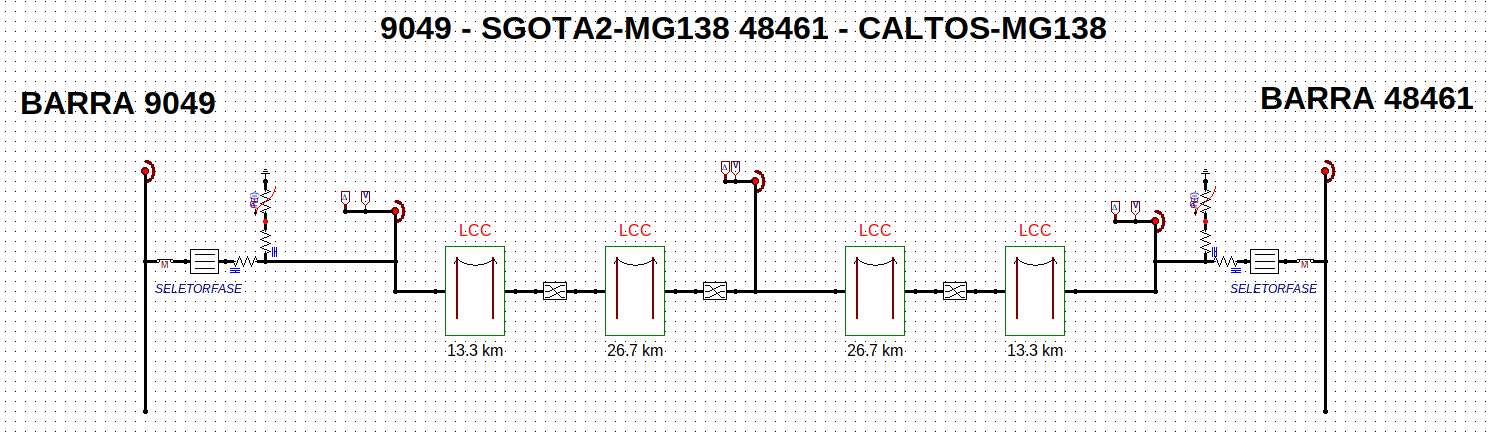
\includegraphics[width=\linewidth,height=3.2cm,keepaspectratio]
    {imagens/modelo_linha_transmissão.png}
  \par\vspace{3mm}
  \begin{tabular}{lll}
    \toprule
    Manobra & Centro da linha & Terminal oposto \\
    $T_{MAN}$ & $1/2\,LT$ & $T_{OPO}$ \\
    \bottomrule
  \end{tabular}
  \par\vspace{3mm}
  \raggedright
  Modelo K.C. Lee não transposto; fases A, B e C.\par
  Passo de integração: $10\,\mu$s. Janela simulada: $0{,}3$ s.
  \source{Fonte: monografia, metodologia e modelo original no ATPDraw.}
\end{frame}

\begin{frame}{Base de dados e unidade de análise}
  \begin{itemize}\setlength{\itemsep}{3mm}
    \item Dois cenários: com resistor de pré-inserção (CRPI) e
      sem resistor de pré-inserção (SRPI).
    \item Cinco tamanhos por cenário: 50, 100, 200, 1.000 e 10.000
      simulações; dez arquivos LIS.
    \item Cada execução fornece nove observações:
      três terminais $\times$ três fases.
  \end{itemize}
  \vspace{2mm}
  \[
    2\times(50+100+200+1.000+10.000)\times9
    =\mathbf{204.300}
  \]
  \takeaway{90 grupos de análise: cenário $\times$ tamanho
    $\times$ terminal $\times$ fase.}
  \source{Unidade de análise: máximo de tensão por execução, terminal e
    fase; não a série temporal da forma de onda.}
\end{frame}

\begin{frame}{Processamento e validação dos dados}
  \begin{enumerate}\setlength{\itemsep}{2mm}
    \item Extrair máximos, instantes e identificadores do LIS.
    \item Verificar identidade, completude e integridade.
    \item Converter os máximos fase-terra:
      \[
        V_{pu}=\frac{|V_{\mathrm{pico,com\ sinal}}|}{112.677\ \mathrm{V}}.
      \]
    \item Calcular estatísticas e preservar a origem dos resultados.
  \end{enumerate}
  \takeaway{204.300 observações mantidas, sem exclusões.}
  \source{60 verificações individuais da fase A e 90 médias do ATP
    concordantes. Cobertura numérica limitada aos pontos declarados.
    Implementação: Python, Polars, SciPy e scikit-learn.}
\end{frame}

\begin{frame}{Critérios de candidatos a anomalias}
  \begin{description}\setlength{\itemsep}{3mm}
    \item[MAD] Escore robusto: $|z_{MAD}|>3{,}5$;
      exige ao menos oito valores finitos e MAD não nulo.
    \item[K-Means] Distância ao centroide atribuído acima do percentil
      99 das distâncias de calibração; $k=2$ na comparação.
    \item[DBSCAN] Pontos de ruído em ajuste aplicável;
      $\varepsilon=0{,}5$ no espaço padronizado e mínimo de cinco vizinhos.
  \end{description}
  \takeaway{Ajustes separados por cenário, fonte, terminal e fase.}
  \source{Rótulos hierárquicos são descritivos e não votantes.
    Diagnóstico gaussiano não seleciona candidatos.
    SIGMAX=3.0 pertence ao chaveamento de entrada do ATP.}
\end{frame}

\begin{frame}{Estatísticas e adequação gaussiana}
  $T_{OPO}$, fase A, 10.000 simulações por cenário.
  \vspace{3mm}
  \begin{center}
    \begin{tabular}{lrr}
      \toprule
      Medida & CRPI & SRPI \\
      \midrule
      Média (P.U.) & 1,1769 & 1,7006 \\
      Desvio padrão amostral (P.U.) & 0,1209 & 0,1317 \\
      Assimetria & 0,7838 & $-1{,}6187$ \\
      Normalidade a 5\% & Rejeitada & Rejeitada \\
      \bottomrule
    \end{tabular}
  \end{center}
  \takeaway{Anderson--Darling rejeitou a normalidade em 88 dos 90 grupos.}
  \source{Fonte: monografia, resultados estatísticos; pacote v9,
    distribution\_adequacy.csv. As duas não rejeições em N=50 não
    comprovam normalidade.}
\end{frame}

\begin{frame}{Distribuição dos máximos: exemplo SRPI}
  \centering
  \includegraphics[width=\linewidth,height=5.1cm,keepaspectratio]
    {\evidence distribution-srpi-t_opo-a.png}
  \source{Fonte: figura da monografia, pacote v9. $T_{OPO}$, fase A,
    N=10.000. Histograma e gráfico quantil--quantil; ajuste normal
    apresentado somente como comparação qualificada.}
\end{frame}

\begin{frame}{Probabilidade empírica de excedência}
  Evento analisado: máximo de tensão acima de $2{,}3$ P.U.
  \[
    \widehat p=\frac{n(V_{pu}>2{,}3)}{N}
  \]
  \begin{itemize}\setlength{\itemsep}{3mm}
    \item Zero excedências nos 90 grupos.
    \item Frequência empírica e intervalo de Wilson de 95\%
      calculados separadamente para cada grupo.
    \item Limite superior: aproximadamente 7,13\% em $N=50$
      e 0,04\% em $N=10.000$.
  \end{itemize}
  \takeaway{Nenhum evento observado não significa probabilidade real nula.}
  \source{Fonte: monografia, resultados probabilísticos; pacote v9,
    probability.tex. O limiar de análise não é recomendação de isolamento.}
\end{frame}

\begin{frame}{Comparação geométrica dos agrupamentos}
  Silhouette maior e Davies--Bouldin menor favorecem separação interna.
  \vspace{3mm}
  \begin{center}
    \begin{tabular}{lc}
      \toprule
      Método & Grupos com índices aplicáveis \\
      \midrule
      K-Means & 90 de 90 \\
      DBSCAN & 4 de 90 \\
      Seleção hierárquica de cauda superior & 6 de 90 \\
      \bottomrule
    \end{tabular}
  \end{center}
  \takeaway{Qualidade geométrica não comprova classes de fenômenos elétricos.}
  \source{Fonte: monografia, comparação de clusterização; pacote v9.
    Índice não aplicável não significa detector não aplicável.
    Ruído excluído pode alterar a população avaliada.}
\end{frame}

\begin{frame}{Candidatos e concordância entre critérios}
  $T_{OPO}$, fase A; denominador de 10.000 por cenário.
  \vspace{3mm}
  \begin{center}
    \begin{tabular}{lrr}
      \toprule
      Critério ou conjunto & CRPI & SRPI \\
      \midrule
      MAD & 109 (1,09\%) & 852 (8,52\%) \\
      Distância do K-Means & 99 (0,99\%) & 99 (0,99\%) \\
      Ruído do DBSCAN & 0 & 0 \\
      MAD $\cap$ K-Means & 99 & 99 \\
      União dos três critérios & 109 & 852 \\
      \bottomrule
    \end{tabular}
  \end{center}
  \takeaway{Concordâncias e discordâncias permanecem explícitas.}
  \source{Fonte: monografia, evidências analíticas; pacote v9,
    method\_comparison.csv. Os três detectores são aplicáveis neste recorte.
    Nenhum candidato foi excluído automaticamente.}
\end{frame}

\begin{frame}{Influência do tamanho amostral}
  Taxa da união de candidatos no CRPI, $T_{OPO}$, fase A:
  \vspace{3mm}
  \begin{center}
    \begin{tabular}{lrrrrr}
      \toprule
      Simulações & 50 & 100 & 200 & 1.000 & 10.000 \\
      \midrule
      Candidatos & 16\% & 12\% & 1\% & 1\% & 1,09\% \\
      \bottomrule
    \end{tabular}
  \end{center}
  \begin{itemize}\setlength{\itemsep}{3mm}
    \item No mesmo recorte SRPI, a taxa varia de 8,52\% a 12\%.
    \item A incerteza da excedência diminui com $N$; a separação
      geométrica não melhora automaticamente.
  \end{itemize}
  \takeaway{10.000 simulações constituem referência empírica,
    sem garantir verdade ou acurácia.}
  \source{Fonte: monografia, comparação amostral; pacote v9.
    As fontes não são presumidas independentes ou aninhadas.}
\end{frame}

\begin{frame}{Ensaios controlados e limites da validação}
  Perturbações pontuais, contextuais e coletivas;
  contaminações de 1\%, 5\% e 10\%, além da condição limpa.
  \vspace{2mm}
  \begin{center}
    \begin{tabular}{lrr}
      \toprule
      Condição limpa & Falsos positivos & Taxa \\
      \midrule
      K-Means & 42 / 5.400 & 0,78\% \\
      DBSCAN por novidade & 391 / 5.400 & 7,24\% \\
      \bottomrule
    \end{tabular}
  \end{center}
  \begin{itemize}\setlength{\itemsep}{2mm}
    \item Vinte réplicas de parâmetros: Jaccard igual a 1 no recorte.
    \item Cinco casos selecionados aguardam revisão elétrica.
  \end{itemize}
  \takeaway{Desempenho sintético e estabilidade não confirmam causa real.}
  \source{Fonte: monografia, avaliação controlada; pacote v9.
    Recorte: CRPI/SRPI, $T_{OPO}$, fase A, fontes de N=10.000;
    divisão por blocos de execução.}
\end{frame}

\begin{frame}{Conclusão e trabalhos futuros}
  \begin{itemize}\setlength{\itemsep}{3mm}
    \item \textbf{Contribuição:} rotina integrada e rastreável,
      executada nos dez arquivos e nas 204.300 observações.
    \item \textbf{Resultados:} candidatos explícitos, probabilidades
      empíricas com incerteza e comparação de métodos.
    \item \textbf{Limite:} causa dos extremos permanece não resolvida.
    \item \textbf{Próximos passos:} formas de onda, repetição com passo
      menor e revisão elétrica independente qualificada.
  \end{itemize}
  \takeaway{A rotina organiza evidências para investigação técnica
    reproduzível.}
  \vspace{2mm}
  \hfill\textbf{Obrigado.}
\end{frame}

\end{document}
